\chapter{Analisi di Ricketts}

Tutte le analisi cefalometriche prevedono l'identificazione di diversi punti craniofacciali. Molti di questi punti sono tradizionali; altri, invece, possono essere specifici di un'analisi in particolare. In questo capitolo si discuterà dell'analisi ideata da Robert M. Ricketts.

\section{Punti cefalometrici}

\paragraph{Condilo (DC)} punto al centro del collo del condilo sul piano \piano{Na}{Ba}.

\paragraph{Centro del cranio (CC)} punto di intersezione del piano \piano{Na}{Ba} con l'asse facciale di Ricketts, che unisce \piano{PT}{Gn}.

\paragraph{CF} punto di intersezione del piano di Francoforte (\piano{Or}{Por}) con la verticale pterigoidea \punto{PTV}, retta perpendicolare al piano di Francoforte passante per il punto \punto{ÞT} e tangente il bordo posteriore della fessura pterigoidea.

\paragraph{Xi} punto geometrico del centro del ramo mandibolare. Per identificarlo, bisogna far riferimento al piano di Francoforte e al PTV, che sono tra loro perpendicolari. Localizzando la parte più interna della concavità anteriore del ramo della mandibola come R$_1$, si traccia da questo una retta parallela al piano di Francoforte, fino al bordo posteriore del ramo della mandibola R$_2$. Si definisce quindi R$_3$ come il punto più basso dell'incisura sigmoidea; facendo partire da questo una retta parallela a PTV, si ricava in basso il punto R$_4$. A questo punto si costruisce un rettangolo, tracciando parallele a PTV e al piano di Francoforte passanti per R$_1$, R$_2$, R$_3$ ed R$_4$. A questo punto si tracciano le diagonali del rettangolo, e il loro punto d'intersezione sarà il punto Xi.

\paragraph{Incision superiore (Is)} è il punto di contatto più basso degli angoli mesiali degli incisivi superiori, corrispondente alla parte più bassa del profilo del bordo incisivo superiore.

\paragraph{Incision inferiore (Ii)} è il punto di contatto più alto degli angoli mesiali degli incisivi inferiori, corrispondente alla parte più alta del profilo del bordo incisivo inferiore.

\paragraph{Pronasale cutaneo (Pn)} è il punto più sporgente della prominenza nasale.

\paragraph{Pogonion cutaneo (Po$_c$)} è il punto più sporgente dell'eminenza mentale.

\section{Analisi craniofacciale}

\begin{figure}[h!]
 \centering
 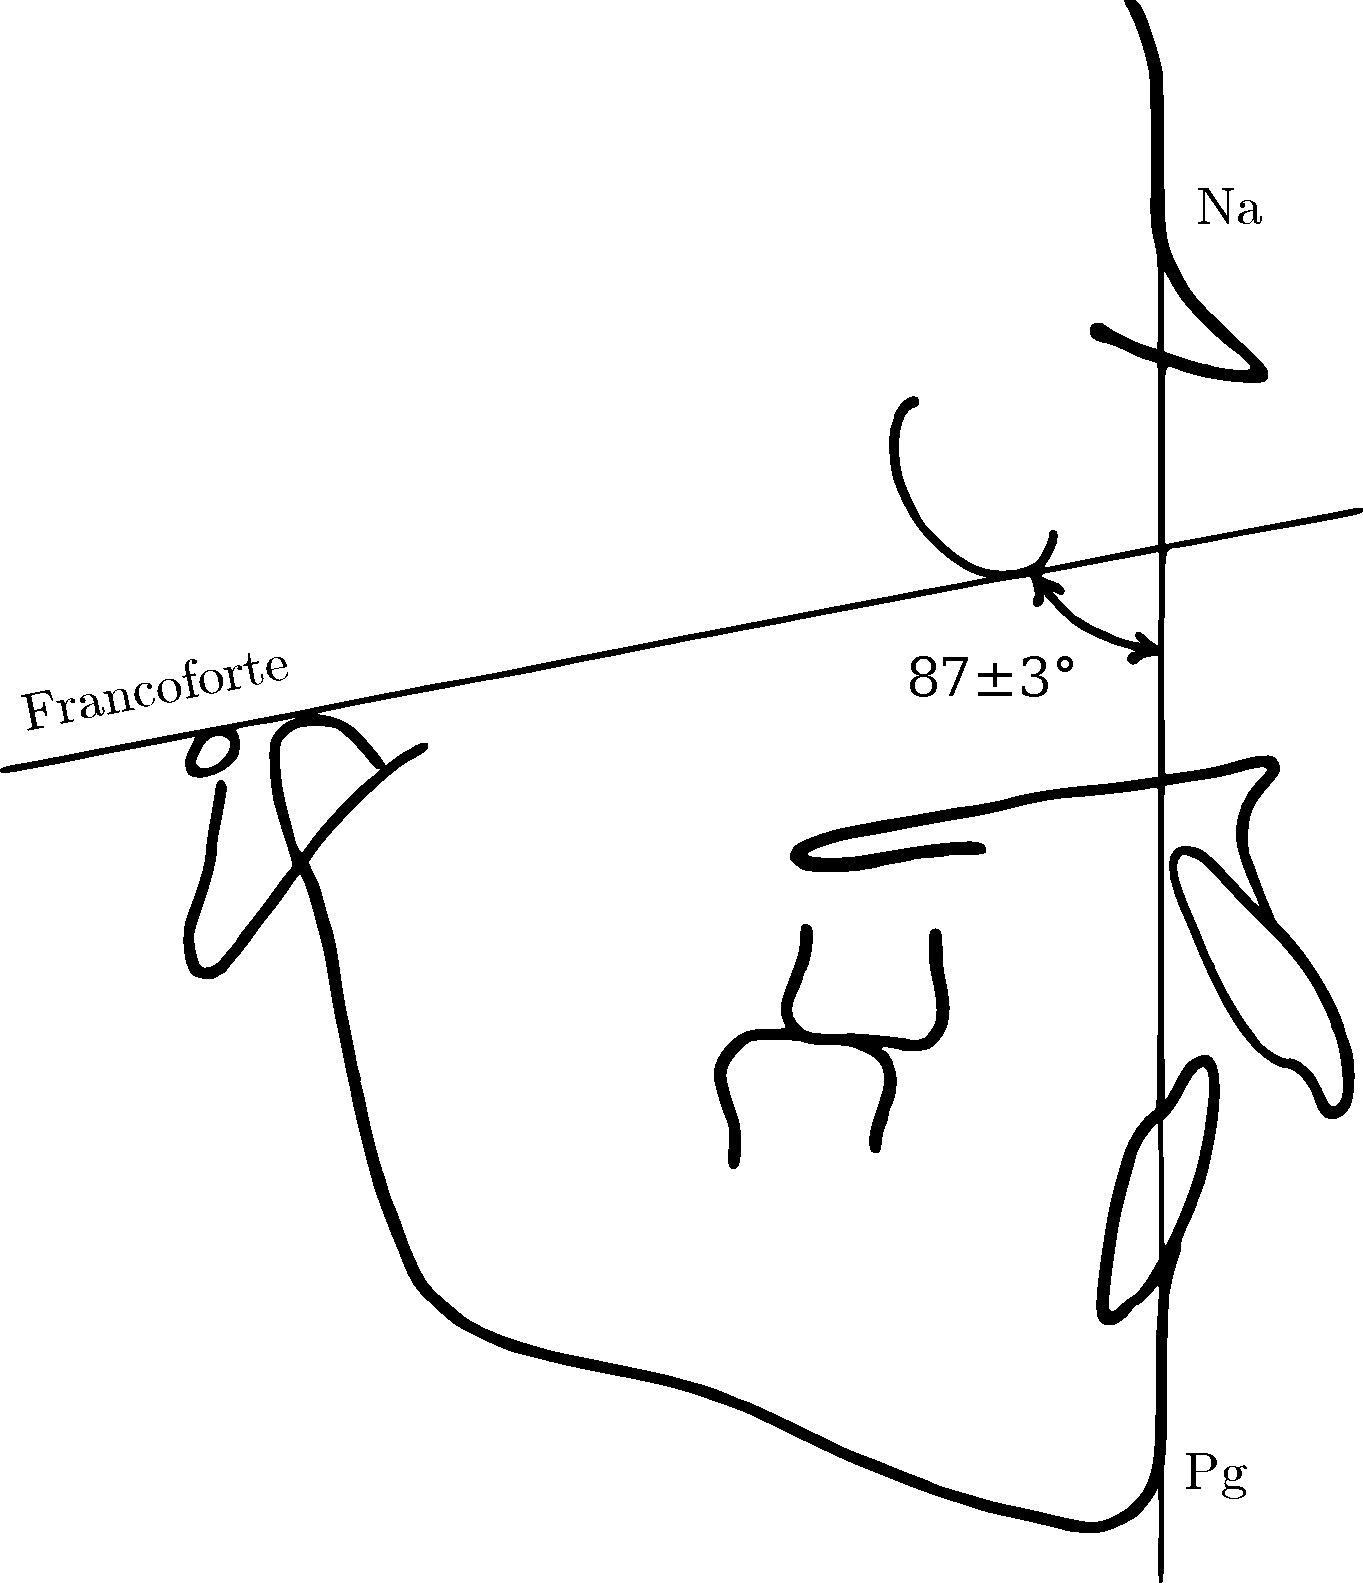
\includegraphics[width=.5\textwidth]{./images/ricketts_facciale_downs.pdf}
 % ricketts_facciale_downs.pdf: 654x760 pixel, 72dpi, 23.07x26.81 cm, bb=0 0 654 760
 \caption{Angolo facciale di Downs}
 \label{fig:ricketts_facciale_downs}
\end{figure}

\paragraph{Angolo facciale di Downs} (fig. \ref{fig:ricketts_facciale_downs}) dato dal piano facciale (\piano{Na}{Po}) col piano di Francoforte, indica la posizione più o meno avanzata della mandibola sul piano sagittale. Il valore medio è 87° a 9 anni, aumenta di 1° ogni 3 anni. La deviazione standard è $\pm$ 3°.

\paragraph{Asse facciale di Ricketts} linea che congiunge il punto \punto{PT} con lo Gnathion. Questa linea forma un angolo con il piano della base del cranio (\piano{Na}{Ba}) nella parte postero-inferiore il cui valore medio normale è di 90°, con una deviazione standard di $\pm$ 3°. Indica la traiettoria di crescita della mandibola: in avanti crescita orizzontale antioraria, in dietro e in basso crescita oraria, in avanti e in basso crescita neutrale; esprime la posizione della mandibola sul piano verticale.

\paragraph{Angolo della conicità facciale} o angolo piano facciale-piano mandibolare: indicativo dello sviluppo in altezza della parte posteriore della faccia. Ha un valore medio di 68°, con una deviazione standard di $\pm$ 4°. Un angolo superiore indica un soggetto ortognatico (brachi-facciale), un angolo inferiore un soggetto prognatico (dolico-facciale).

\paragraph{Angolo piano di Francoforte-piano mandibolare} esprime il grado di inclinazione mandibolare, e la posizione verticale della mandibola. Ha un valore medio di 26°, che diminuisce con l'età, con una deviazione standard di $\pm$ 4°. Un angolo superiore indica un soggetto prognatico (dolico-facciale), un valore inferiore un soggetto ortognatico (brachi-facciale).

\paragraph{Angolo piano di Francoforte-piano \piano{Na}{A}} è la profondità mascellare, indica la posizione più o meno avanzata del mascellare superiore sul piano sagittale. Ha un valore medio di 90° $\pm$ 3°.

\paragraph{Angolo piano \piano{Na}{CF} con il piano \piano{CF}{A}} è l'altezza mascellare superiore, indica la posizione del mascellare superiore sul piano verticale. Ha un valore medio di 54°, che aumenta di 1° ogni 3 anni. La deviazione standard è $\pm$ 3°.

\paragraph{Angolo piano di Francoforte con il piano bispinale} è indicativo dell'orientamento del mascellare superiore verso l'alto o verso il basso. Ha un valore medio di 1° $\pm$ 3°.

\paragraph{Angolo \piano{Na}{Ba} con il piano di Francoforte} angolo supero-anteriore, esprime il grado di inclinazione della base cranica. Ha un valore medio di 26° $\pm$ 2°. Valori superiori indicano una crescita verso il basso del Basion (crescita antioraria); valori inferiori indicano una crescita in dietro del Basion (crescita oraria).

\paragraph{Lunghezza base cranica anteriore} misurata tra il punto \punto{CC} e il punto \punto{Na}. Ha un valore medio di 56 $\pm$ 3mm a 10 anni, e aumenta di $0,8$ mm ogni anno. Valori superiori indicano che il soggetto è di tipo prognatico (dolico-facciale), valori inferiori che il soggetto è ortognatico (brachi-facciale).

\paragraph{Altezza facciale posteriore} distanza \punto{CF}-\punto{Go}, ha un valore medio di 56 $\pm$ 4mm. Valori superiore indicano un aumento in altezza del ramo mandibolare, valori inferiori ne indicano un accorciamento.

\paragraph{Posizione del Porion} distanza tra il Porion e il piano pterigoideo verticale. Valore medio di 39 $\pm$ 2mm, aumenta di $0,5$mm per anno.\footnote{FIXME: a che età è la media?}

\paragraph{Angolo piano \piano{CF}{Xi} con la linea verticale pterigoidea} dà la posizione del ramo mandibolare, ha un valore medio di 15 $\pm$ 3°. Valori superiori indicano una crescita posteriore della mandibola, valori inferiori una crescita anteriore.

\paragraph{Angolo dell'arco mandibolare} formato dal prolungamento dell'asse del corpo mandibolare con l'asse condilare. Il valore medio è di 27 $\pm$ 5° a 9 anni; valori superiori indicano che la mandibola è orientata orizzontalmente, mentre valori inferiori indicano che la mandibola è orientata in basso e indietro, cioè il corpo mandibolare è molto inclinato.

\paragraph{Lunghezza del corpo mandibolare} è data dalla distanza \punto{Pm}-\punto{Xi}. Il valore medio è di 66mm a 9 anni, con un range di variazione dai 64 ai 70mm. Indica il grado di sviluppo mandibolare: valori inferiori indicano che la mandibola è corta, valori superiori indicano una mandibola lunga.

\section{Analisi del sistema scheletrico}
\paragraph{Convessità} è data dalla distanza del punto \punto{A} dal piano facciale. Valori medi normali sono da 3 a 5mm, con una deviazione standard di $\pm$ 2mm. La convessità è indicativa della posizione del mascellare superiore in rapporto alla mandibola. Essa è positiva quando il punto \punto{A} è anteriore al piano facciale, e indica un modello scheletrico di Classe II. È invece negativa quando il punto \punto{A} è posteriore al suddetto piano, e indica un modello scheletrico di Classe III. La convessità diminuisce con l'età, soprattutto in pazienti con un buon potenziale di crescita orizzontale.

\paragraph{Altezza facciale inferiore} è data dal valore dell'angolo \punto{SNA}-\punto{Xi}-\punto{Pm}, il cui valore medio normale è di 47 $\pm$ 4°. Quest'angolo non si modifica con la crescita.

\section{Analisi dentale}

\paragraph{Relazione dei molari sul piano sagittale} viene calcolata la distanza tra le superfici distali dei primi molari superiori ed inferiori, misurati sul piano occlusale. Valori medi sono:
\begin{itemize}
\item Classe I: -3mm;
\item Classe II: 0mm o maggiore;
\item Classe III: -6mm.
\end{itemize}

Valori negativi sono indicativi di una posizione distale dei molari superiori rispetto agli inferiori.

\paragraph{Relazione dei canini sul piano sagittale} è data dalla distanza tra le cuspidi dei canini misurata sul piano occlusale.
\begin{itemize}
\item Classe I: -2 $\pm$ $0,7$mm;
\item Classe II: +1mm;
\item Classe III: -5 $\pm$ 3mm.
\end{itemize}

\paragraph{Rapporto tra incisivi superiori ed inferiori sul piano antero-posteriore (\textit{overjet})} distanza sagittale dei margini incisivi misurata sul piano occlusale. Valore medio $2,5$ $\pm$ $2,5$mm.

\paragraph{Rapporto verticale tra incisivi superiori ed inferiori (\textit{overbite})} distanza verticale tra i margini incisivi, misurata perpendicolarmente al piano occlusale. Valore medio $2,5$ $\pm$ 2mm.

\paragraph{Angolo interincisivo}, formato dagli assi degli incisivi. Valore medio 130 $\pm$ 6°. Per i soggetti prognatici il valore normale varia da 115° a 125°, per i soggetti ortognatici da 135° a 145°.

\section{Rapporti dento-scheletrici}

\paragraph{Posizione del primo molare superiore} data dalla distanza tra la superficie distale del sesto superiore e il piano pterigoideo verticale. Il valore medio normale è uguale all'età del paziente $+$ 3 $\pm$ 3mm.

\paragraph{Posizione dell'incisivo inferiore in relazione ai mascellari} data dalla distanza del margine incisale inferiore dalla linea \piano{A}{Po}, con un valore medio di $2,4$ $\pm$ 2mm. La misura è positiva quando l'incisivo è davanti alla linea \piano{A}{Po}, negativa quando è indietro.

\paragraph{Inclinazione dell'incisivo inferiore} misurata dall'angolo che l'asse incisivo inferiore forma con la linea \piano{A}{Po}. Ha un valore medio di 22 $\pm$ 4°; valori superiori indicano un tipo scheletrico prognatico (dolico-facciale), valori inferiori un tipo ortognatico (brachi-facciale).

\paragraph{Inclinazione dell'incisivo superiore} misurata dall'angolo che l'asse incisivo superiore forma con la linea \piano{A}{Po}. Ha un valore medio di 28 $\pm$ 4°, e dev'essere parallelo all'asse facciale.

\paragraph{Inclinazione del piano occlusale} è data dall'angolo che il piano occlusale forma con l'asse del corpo mandibolare. Ha un valore medio di 22° a 8 anni e 20° a 12 anni, e diminuisce di $0,5$° ogni anno. Ha una deviazione standard di $\pm$ 2°.

\section{Analisi estetica}

\paragraph{Rapporto del labbro inferiore con la linea estetica E di Ricketts} il cui valore medio è $-$2 $\pm$ 2mm. Con il labbro in posizione normale va da $-$2 a 0mm. Il labbro si dice retruso se è oltre i $-$3mm, altrimenti è protruso oltre i 3mm.
